\chapter{Overzicht van het thera project}
\label{hoofdstuk:overzicht}
Zoals eerder gezegd bouwt deze thesis verder op een reeds bestaand project. Om ze beter te kunnen situeren in het geheel is het handig om eerst even het thera project bekijken
en dan te zien waar dit project in past.

\section{De opdelingen van het thera project}
Ruwweg gezien kan het reconstrueren van een fresco met behulp van de computer opgedeeld worden in 3~fasen.

\begin{description}
	\item[Acquisitie] Alle gevonden fragmenten worden ingescand met behulp van 3D en 2D-scanapparatuur om zo een virtueel model van elk stuk te bouwen, zie \cite{Brown2008}.  
	\item[Identificatie] Vervolgens worden deze virtuele fragmenten aan een zogenaamde \emph{matcher} gegeven, die voor elk fragmentenpaar gaat kijken of ze mogelijk op elkaar passen. Er zijn verschillende types ontwikkeld, waarvan \'e\'en van de meeste succesvolle de zogenaamde \emph{RibbonMatcher} \cite{Brown2008} bleek te zijn. Deze \emph{matcher} kijkt enkel naar de randen van de fragmenten en kan dus zelfs volledig kleurloze fragmentparen identificeren. Maar het onderzoek gaat verder, in 2010 werd er een nieuw type ontwikkeld dat zijn analyse baseert op een combinatie van verschillende eigenschappen, zoals de sporen die een borstel kan nalaten bij het kleuren van een fresco \cite{TolerFranklin2010}.
	\item[Classificatie \& Reconstructie] De laatste stap bestaat uit het classificeren van wat de vorige stappen produceren (en zodoende het samenstellen van een fresco). Elk voorgesteld paar moet gecontroleerd worden op validiteit. Verschillende statussen kunnen zo toegekend worden aan
	een paar, zoals: \emph{geconfirmeerd}, \emph{misschien}, \emph{nee}, \emph{conflict}, et cetera. De \emph{matcher} produceert namelijk zeer veel mogelijk passende paren, waarvan slechts een klein deel correct zal zijn. De drempel voor het beslissen wat een paar kan zijn en wat niet wordt in de \textbf{identificatie}-stap zo laag ingesteld omdat men wil vermijden dat twee fragmenten die toch passen genegeerd worden (de kost van zogenaamde ``\emph{false negatives}'' wordt hoog ingeschat).
\end{description}

\section{Reconstructie, de bestaande oplossingen}
Het thesisproject besproken in deze tekst tracht de reeds bestaande hulpmiddelen van de reconstructiefase aan te vullen. Hievoor werden reeds programma's ontwikkeld, namelijk \emph{Griphos} en \emph{Browsematches}. Hierop volgt een bondige bespreking van beide programma's, wat ze kunnen en niet kunnen, en eventuele voor- en nadelen. Deze factoren hebben een belangrijke rol gespeelt in de richting van dit thesisproject.

\subsection{Griphos}

Griphos was het eerste programma gericht op het weergeven en beoordelen van de resultaten van de voorgaande stappen. Het werd ontworpen met het doel een centraal zenuwstelsel te zijn voor alle informatie en met deze uiteindelijk een (zo goed mogelijk) gereconstrueerd fresco te maken. Men kan er zowel aparte fragmenten als fragmentparen ge\"identificeerd door een algoritme op een virtueel tafelblad plaatsen en manipuleren. De idee achter een dergelijke voorstelling komt natuurlijk voort uit een rechstreekse vertaling van wat een archeoloog doet op een werkelijk tafelblad naar de computer.\\

\begin{figure}[ht]
	\begin{center}
		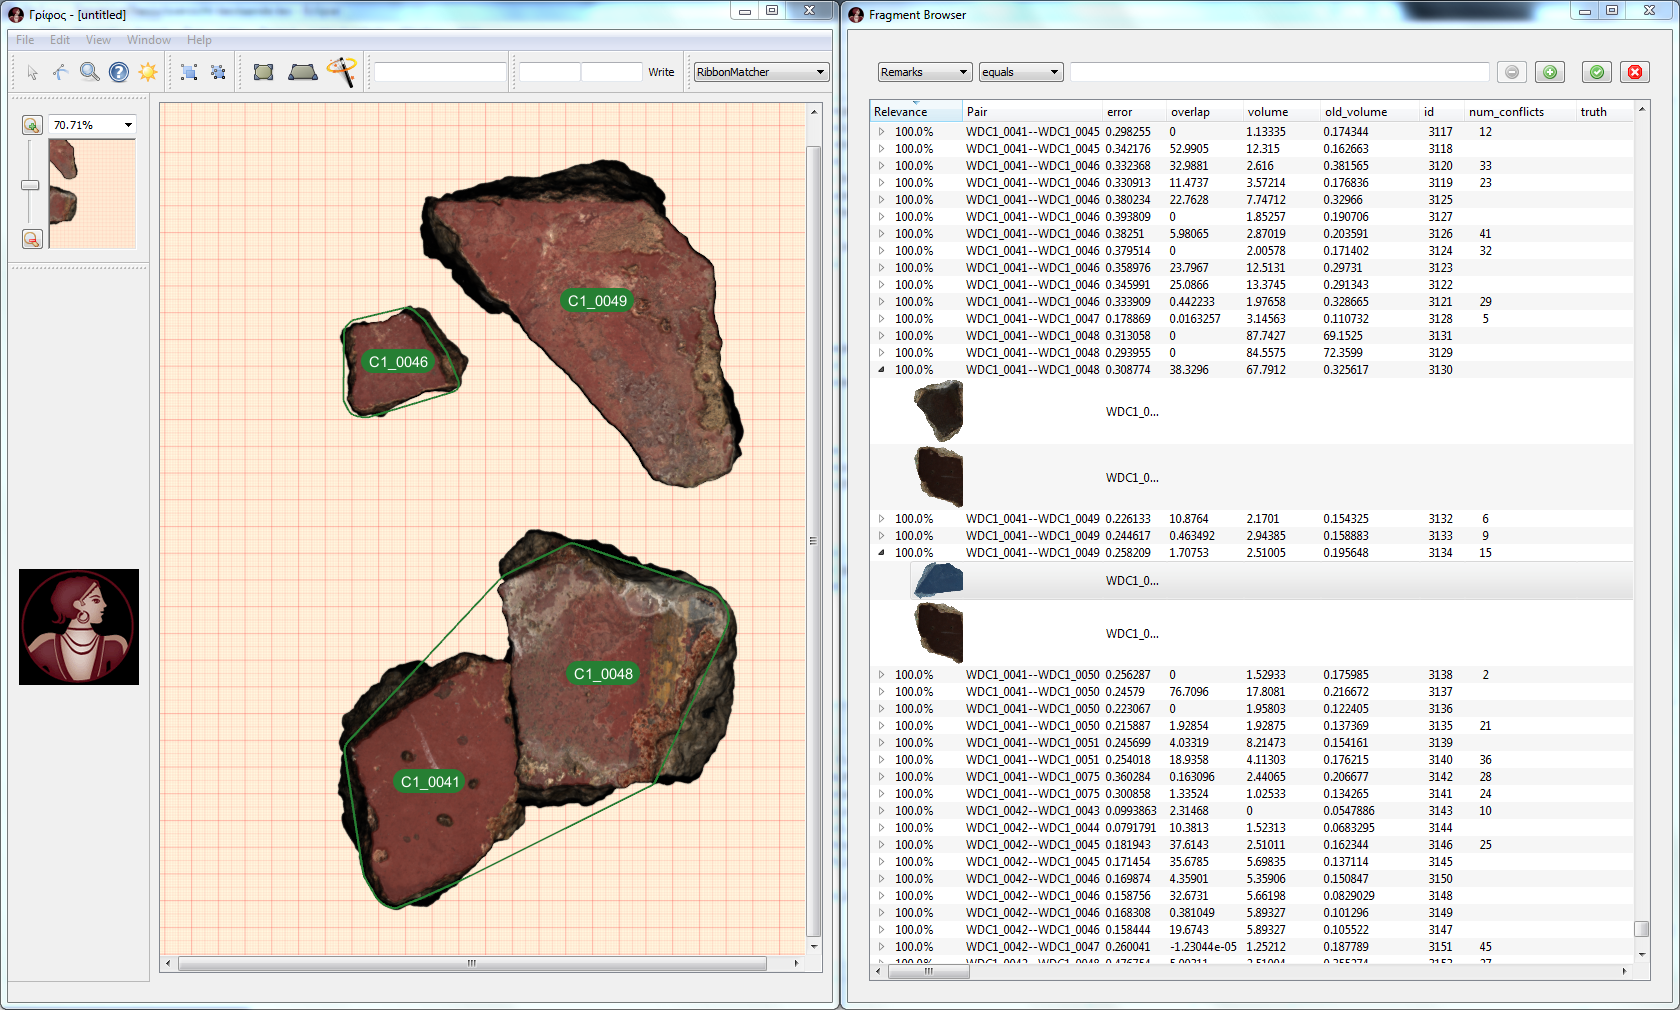
\includegraphics[width=.8\columnwidth]{images/griphos-01-cut.png}
		\caption{Een voorbeeld Griphos tafelblad, 1 voorgesteld paar en 2 aparte fragmenten zijn reeds ingeladen}
	\end{center}
\end{figure}

Het programma wordt echter geplaagd door een paar problemen: het is traag en biedt geen goede wijze aan om de (honderd-)duizenden gegenereerde paarvoorstellen na te kijken. De gebruikte metafoor van het virtuele tafelblad waarin gepuzzeld kan worden stelt weliswaar een belangrijk deel van het reconstructieproces voor, maar schiet tekort als men de nieuwe computergestuurde technieken van fragmentpaar-ontdekking op vloeiende wijze in het proces wil betrekken. Het probleem lijkt te zijn dat er te veel informatie is, en Griphos geen goede manier aanbiedt om door de bomen het bos te zien. De aanzienlijke traagheid van sommige delen van het programma komen vooral voort uit het statische en niet-schaalbare datamodel voor paren (XML bestanden) en de complexiteit van de visualisatie (afbeeldingen van hoge kwaliteit en gedetailleerde 3D-modellen). Dit zorgt voor een soms onaangename werkervaring zelfs indien men er toch in slaagt de juiste fragmentparen te lokaliseren. Desalniettemin is het een krachtig programma dat veel functionaliteit biedt voor de detailinspectie van brokstukken.\\

Het heeft zijn nut al op verschillende vlakken bewezen, behalve detailinspectie is het bijvoorbeeld ook in staat om de posities van fragmenten in een bak te onthouden. Dit betekent een grote snelheidswinst wanneer men bijvoorbeeld denkt een goed paar te hebben gevonden en men wil dit met echte fragmenten verifi\"eren. Als beide fragmenten in dezelfde bak liggen kan het correcte tafelblad ingeladen worden, Griphos kan vervolgens de gezochte fragmenten laten oplichten. Hetgeen veel gemakkelijker is dan zelf te zoeken door de vormen te vergelijken, zeker omdat de brokstukken vaak moeilijk te onderscheiden zijn zoals te zien valt in figuur \ref{fig:griphosbak}. 

\begin{figure}[ht]
	\begin{center}
		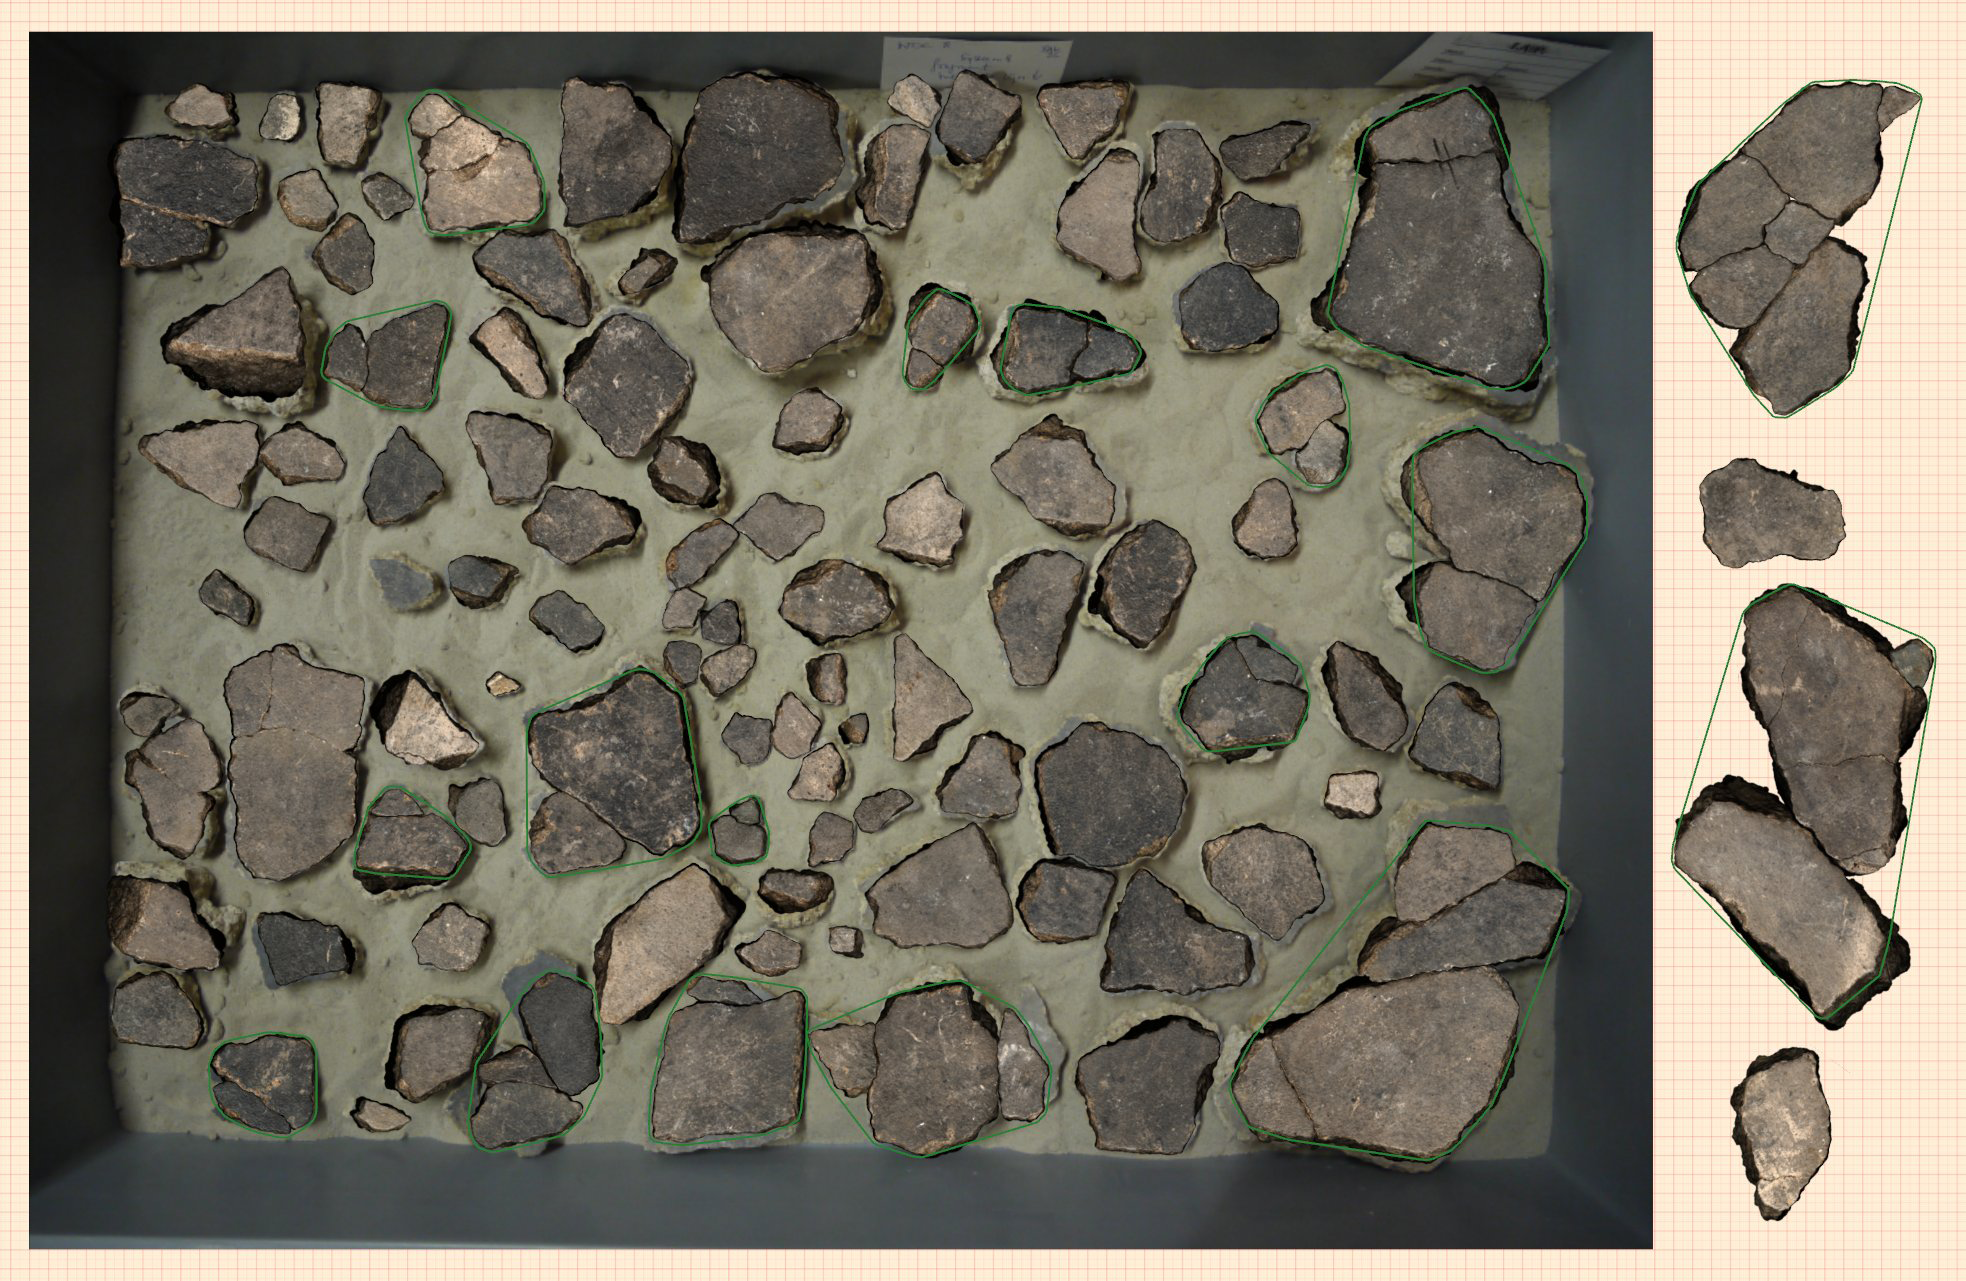
\includegraphics[width=.8\columnwidth]{images/griphos-bak-01.png}
		\caption{Griphos kan gebruikt worden om de posities van fragmenten in hun opslagplaats te onthouden en vervolgens snel terug te vinden. De brokstukken die buiten de bak staan weergegeven zijn verplaatst geweest naar een andere bak. (afbeelding met toestemming gebruikt uit \cite{Brown2011})}
		\label{fig:griphosbak}
	\end{center}
\end{figure}

// te technisch voor dit hoofdstuk, verplaats naar iets later: [TODO: remove]
Het eerste probleem wordt vooral veroorzaakt door trage datatoegang en te complexe visualisaties. Het programma slaagt alles betreffende paren op in een (enorm) XML bestand. Dit is nog doenbaar als men slechts een paar duizend voorstellen heeft maar ondervindt reeds snel onacceptabele vertragingen eens men er meer probeert in te laden. Ter voorbeeld, een kleine voorstellenverzameling van een bepaalde opgraving heeft er reeds 50000. Gekoppeld hieraan laadt Griphos ook steeds een hoge-kwaliteits afbeelding of zelfs een volledig 3D-model in voor elk paar De combinatie van het gebruik van grote XML-bestanden om informatie over de paren in op te slaan, en het steeds inladen van hoge kwaliteits-afbeeldingen en 3D-modellen. om alle info in op te slaan. Dit is bijzonder innefici\"ent en geeft ook bitter weinig mogelijkheden tot uitbreiding. Een ander deel is het gebrek aan zoekmogelijkheden binnen de voorstellen.

\subsection{Browsematches}

Een eerste prototype om de in Griphos ontbrekende delen aan te vullen, werd Browsematches genoemd. Het gebruikte eerst de visualisatiecapabilitieiten van Griphos om kleine afbeeldingen te nemen van elk bestaand paar samen met aan de linkerkant de doorsnede van hun raakvlak, en probeerde er vervolgens zo veel mogelijk te tonen. \\

\begin{figure}[ht]
	\begin{center}
		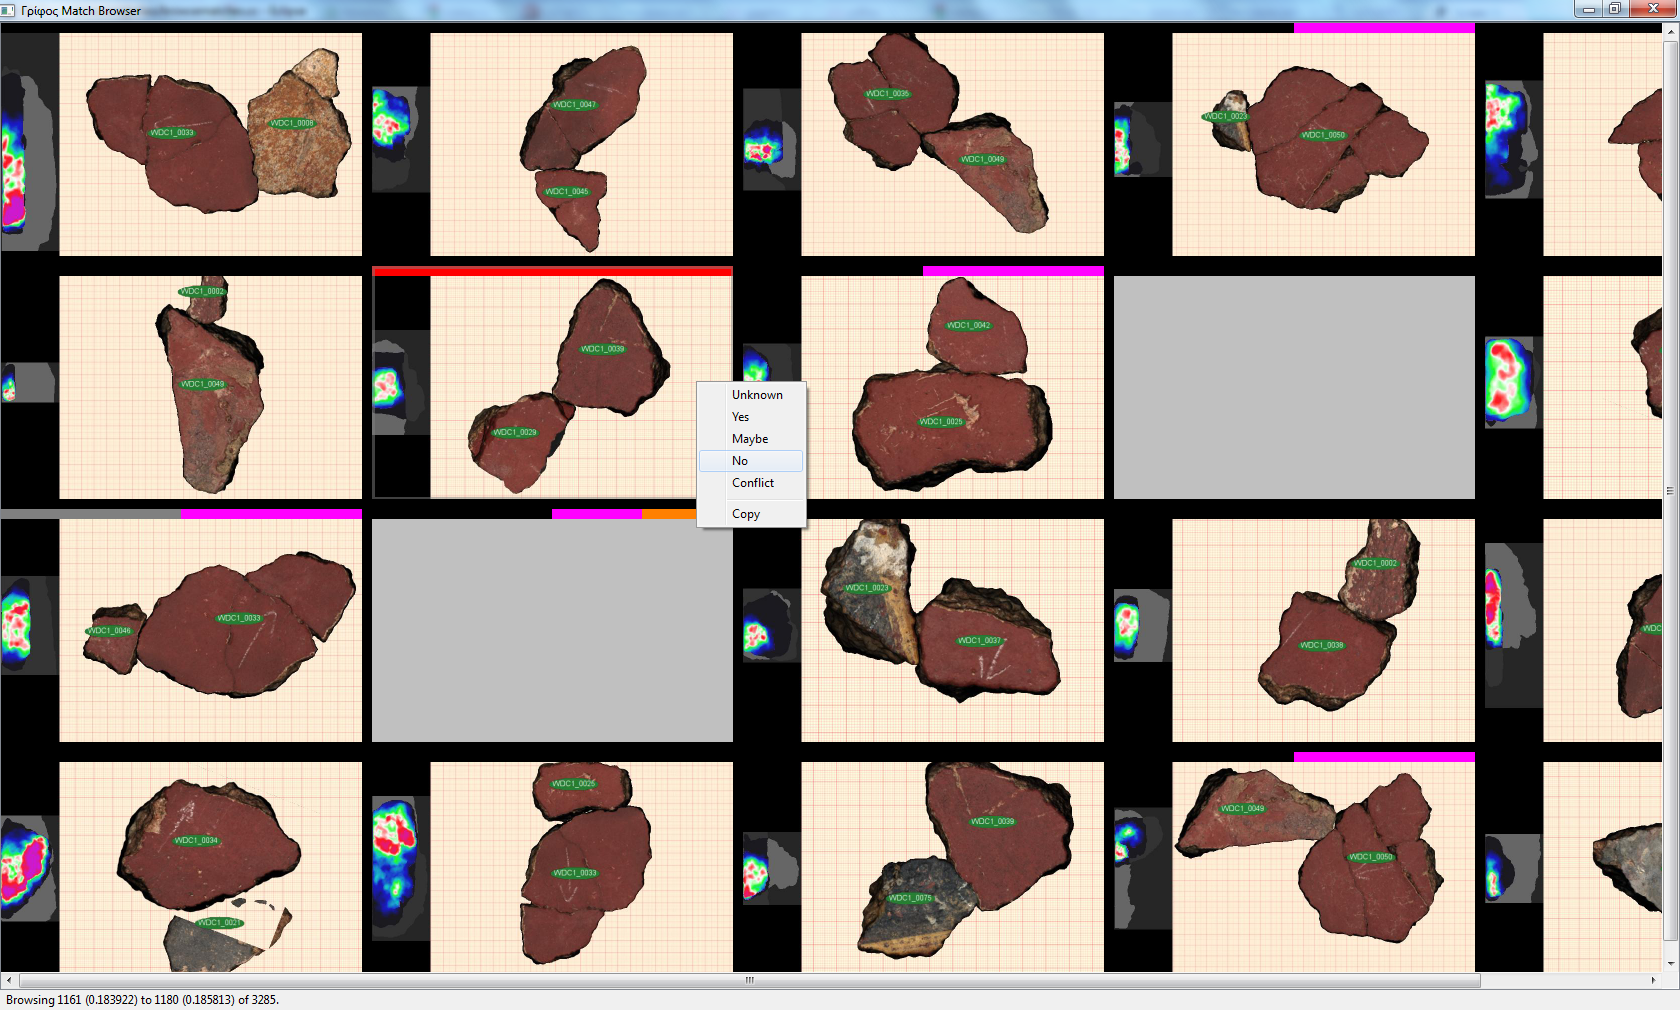
\includegraphics[width=.8\columnwidth]{images/browsematches-01-cut.png}
		\caption{Browsematches in werking, de balken boven de paren duiden een validatie door de gebruiker aan. Rood betekent bijvoorbeeld ``dit voorstel is zeker niet juist''}
	\end{center}
\end{figure}

Dit kleine programma groeide uit noodzaak: het valideren van paarvoorstellen was zo omslachtig met Griphos dat Browsematches in korte tijd in elkaar werd gestoken en met veel succes werd gebruikt om het proces te stroomlijnen. Bij het begin van de thesis, bij wijze van kennismaking met het thera project, werd een verbinding gemaakt met Griphos zodat voorstellen die interessant waren in detail bestudeerd konden worden.\\

Browsematches erfde echter ook enkele van de nadelen van Griphos. [TOOOOOOOOODOOOOOOOOOOOOOO]Het datamodel schaalde nog steeds niet goed, was moeilijk uitbreidbaar en deelbaar en mistte doorzoekbaar, gemakkelijk uitbreidbaar of deelbaar. Daarenboven was het programma slechts een prototype en niet bedoeld voor algemeen gebruik. Het simpele maar succesvolle concept diende als inspiratie en basis voor deze thesis. 

%%% Local Variables: 
%%% mode: latex
%%% TeX-master: "masterproef"
%%% End: 
